\documentclass[12pt,a4paper]{article}
\usepackage{ucs}
\usepackage{caption}
\usepackage[latin1,utf8x]{inputenc}
\usepackage{amsmath}
\usepackage{caption}
\captionsetup{font=small,labelfont=bf}
\usepackage[danish]{babel}
\usepackage[rmargin=3cm,tmargin=3.3cm]{geometry}
\usepackage{listings}
\usepackage{color}
\setlength{\parindent}{0pt}
\setlength{\parskip}{1ex plus 0.5ex minus 0.2ex}
\usepackage{graphicx}
\usepackage{fixltx2e}

\usepackage[T1]{fontenc}
\usepackage{textcomp}


%insert links
\usepackage{hyperref}
\usepackage{fancyhdr,lastpage}	
\pagestyle{fancy}


\definecolor{mygreen}{rgb}{0,0.6,0}
\definecolor{myblue}{rgb}{0,0,1}
\definecolor{myyellow}{rgb}{0.7,0.7,0}
\definecolor{myblack}{rgb}{0,0,0}

\lstset{
	basicstyle=\ttfamily\footnotesize
	breaklines=true,
	numbers=left, 
	commentstyle=\color{mygreen},
	stringstyle=\color{myyellow},
}

%header
\lhead{ 
	Embedded Systems A2\\
	02131 \\ 
}
\chead{ 
}
\rhead{ 11 November, 2013 \\ \bigskip  }

%Footer
\lfoot{
	\rule{\textwidth}{0.1mm}\\
}

\cfoot{}
\rfoot{\ \\ \scriptsize{Side \thepage\ af \pageref{LastPage}}}

\begin{document}

%Forside
\begin{titlepage}
	\begin{center}
		\vspace*{13\baselineskip}
		\huge
		\bfseries
		Embedded Systems\\ 
		\ \\
		02131 \\[5\baselineskip]

		\normalfont
		\Large
		R-peak detection. \\
		Assignment 2\\	
		2013

		\small
		\vfill
	\end{center}	
	\begin{flushleft}
		Jakob Welner, s124305\\
	 	Jacob Gjerstrup, s113440\\
	\end{flushleft}
\end{titlepage}

\ \\
\section*{Abstract}
The task of this assignment was to implemented, integrate and analyse a co-processor. This co-processor would be taking care of a very specific task that was defined by analysing what \"good performance\" means for this task. It was be implemented in such a way that it could communicate with a processor through a bus, the processor being the master and the co-processor being the slave. Once it was implemented and integrated, its performance were analysed to determine the improvement in performance, thereby finding out that it does have \"good performance\" as defined earlier.\\
\textbf{May need to be updated!}

\thispagestyle{empty} 
\newpage

%Table of Contents
\tableofcontents
\thispagestyle{empty} 
\newpage

%Reset pagecount
\setcounter{page}{1}

%Alm. sider
\ \\
\section{Introduction}
	After successfully implementing and integrating a dedicated processor to take care of the MWI filter, Medembed wants a co-processor implemented and integrated into the same system. The task of this co-processor would be to further optimize the algorithm, letting the processor created in A2 take care of the more general tasks while the co-processor takes care of a very specific task with a minimum of power, time and size required.\\
	This co-processor were to be implemented in Gezel like the initial processor, and this report will discuss precisely how this co-processor were developed and integrated. It will also discuss what is most important in terms of performance, that is, whether the co-processor is implemented with optimizing speed, power or size in mind.\\
	
\subsection{Requirements}
Below follows a list of functional and non-functional requirements:\\

\textbf{ Functional requirements for the application:}
\begin{itemize}
	\item A co-processor must be designed. This co-processor must be analysed in terms of:
	\begin{itemize}
	\item Functionality
	\item Communication interface
	\item Performance (Speed, area and power)
	\end{itemize}
	\item The co-processor must be implemented and integrated into the system with the processor and RAM
	\item The co-processor must communicate with the processor and RAM through a bus.

\end{itemize}
\textbf{Non-functional requirements for the application:}
\begin {itemize}
	\item The co-processor must be implemented with the use of Gezel
\end{itemize}

\section{Analysis}
 	In order to initiate the structure- and design-process of the program, a number of questions needed to be answered first:\\
 	
 	\begin{enumerate}
	\item How do we define ``good performance''?
	\item What functionality should the co-processor have?
	\item How should the co-processor communicate with the rest of the system?
	\item How can the co-processor be implemented?
	\item How can the co-processor be integrated into the system?

\end{enumerate}

\subsection{Problem 1: Defining good performance}
	The first thing that should be done would be to analyse the co-processor in terms of what good performance is. In terms of performance, there are three areas to consider, and these are: High speed, low area and low power. The task was to decipher which was more important for the current project, as each has a distinct impact on the co-processor.\\
	
	\subsubsection{Speed}
	The impact of speed is that if the co-processor is not fast enough, data will get bogged down and the user will be shown incorrect or old data - therefore, speed is important. A way to increase the speed would be to increase the amount of transistors on the device, but that will increase both size and power.\\
	Furthermore, whereas the speed of a processor is usually calculated in clock cycles (2.8 GHz is 2.8 million clock cycles per second, for instance), clock periods should be used instead.\\
	This is because clock cycles has no definite time period associated with them, and as such, two quick clock cycles can be faster than 1 long clock cycle. An example of this could be 2 additions and one \& operation that takes 3 clock cycles but only 6 ns, whereas a multiplication followed by a division (also two clock cycles) might take 10 ns.\\
	A clock period is the time it takes for two processes to process through a critical path - that is, to do calculations that other parts of the processor depends on. In the previous example of 2 additions and 1 \& operation in one process, and the other process has a multiplication and a division, the clock period of these two processes would be equivalent to the longest period of the two, and therefore, the clock period = 10 ns.\\
	
	\subsubsection{Power}
	Power is important as it will either have the impact that the user will need to charge the battery more often, which will be a hazzle, or that the size of the battery will increase, thus increasing the total size of the device.\\
	To measure the power of a chip, three values can be considered - the first is switching, which is the amount of power used because of active components; the second is short-circuit, which is when both pMOS and nMOS are on at the same time\footnote{Insert reference for explanation}; and the final value is called static and refers to power supply due to inactive components. This report will focus mainly on switching, as this value rise proportionally with activity, and this can be measured by looking at the amount of toggles that happens within a program - that is, the amount of signals switching from 0 to 1 or from 1 to 0.\\
	
	\subsubsection{Size}
	Finally, size is important as the larger the co-processor is, the larger the whole unit will become and finally, the more cumbersome it will be to use in a day-to-day life.\\
	Size can be measured by simply counting the amount of components and bitwidths and adding all these together.
	\\
	
	
\subsection{Problem 2: Functionality of the co-processor}
	Once the choice of performance requirement had been chosen, the next task was to decide how to actually optimize the co-processor in terms of that specific task. There were two ways to implement equation 1 \footnote{See 	\cite{A3}, page 2 for the equation} :\\
	One way was to sum all the values first and then divide with N. The other was to divide every valuable with N before summing them up. Both ways are correct, mathematically speaking, but the way each calculation is done is very different, and it would be important to identify the benefits and issues with choosing 1 over the other in regards to the choice of performance requirement.\\
	
\subsection{Problem 3: Communication of the co-processor}
	The next task was then to identify a suitable communication interface. This interface had to be able to handle transferring of the filtered data from the memory to the co-processor, as well as a way of deciding when the co-processor should begin and stop executing.\\
	The task here was then to define the above, and furthermore, to prepare a list of commands that the co-processor has to be able to carry out to do the calculation of the equation, followed by drawing a block diagram of how exactly the communication interface will work.

\subsection{Problem 4: Implementation and integration of the co-processor}
	Once the previous steps had been taken care of, the next part was to then implement a co-processor and subsequently integrate this into the system developed in A2. The actual implementation were very straight forward and thus did not give any problems, but the integration turned out to be more troublesome.\\

\section{Design}



	
\section{Implementation}
\subsection{Good Performance}
	\subsubsection{Speed}
	Speed remains important as the processor must be able to process the necessary 250 data points per second that the sensor picks up, as if it cannot manage this, the incoming data will be delayed more and more, and the user will be shown old data. However, once this threshold has been passed, speed becomes the least important part, as if it runs much faster than necessary, it will simply idle as it waits for data points, wasting power on nothing. This report deems speed to be the most important, at least up to the point where it can calculate 250 data points per second, simply because the processor must be able to do these calculations and the harder it is to do these calculations, the larger the processor will be (increasing size) and the more power it will require (increasing power consumption). The opposite naturally also holds - the faster the processor is beyond 250 data points, the smaller it can be made, and the lower the clock frequency can be set, thus reducing both size and power.\\
	
	\subsubsection{Power and Area}
	Opposite speed, power and area both remains unimportant until the threshold of 250 data points has been reached, at which point they become much more important. Furthermore, as was documented in A2, reaching 250 data points per second in terms of speed is not a hard feat, and as such, for the purpose of defining what \"good performance\" means, power and area remains more important than speed.\\
	\\
	Of these, this report deems that power remains slightly more important for the following reasons:\\
	\begin{enumerate}
	\item If the processor is too big, the ECG scanner becomes unwieldy and cumbersome, not to mention that current manufacturing processes of general purpose processors are now able to make the devices very small, making it harder to justify why a dedicated chip should be produced.
	\item If the device requires too much power, the processor will either need to be charged more often (which a user can live with, but it is bothersome) or, if taken further, the user might need to change batteries in the middle of the day. The alternative is to increase the size of the battery to make up for the power consumption, but as that increases the size of the device, the risk is that it becomes too unwieldy and cumbersome to use in a day-to-day life.
	\end{enumerate}
	Therefore, optimizing in terms of power will both keep the power consumption down and keep the battery from requiring too much space, thus not increasing the size of the device.\\
	
\subsection{Functionality of the co-processor}
	\label{Functionality}
	With the considerations above in mind, the functionality of the co-processor should now be defined. This report decided to only divide after everything has been summed up, as having a division for each value to be summed would not only slow the processor down greatly (A division involves a multiplication and a bitshift, and whereas a bitshift is quite fast, a multiplication is not), it would also mean more mathematical operations per data sample, which in turn would mean the amount of toggles would be higher, thus increasing the power consumption as well.\\
	\\
	Furthermore, as in A2, it was decided not to sum up all 30 values for every single data point - instead, a variable will hold the value of the 30 previous points and when a new data point is loaded, it will be added to the summation variable and the value that goes 30 data points backwards will be subtracted. This means that instead of adding 30 variables, all that needs to take place is a single addition and a single subtraction, and since addition and subtraction are almost equally as fast, this is certainly a benefit, speedwise. Furthermore, it also cuts down on the amount of toggling, as the processor only needs two points, rather than 30, to do the calculations.\\
	\\
	The above is made possible by sending all data in a single 32 bit signal over the bus - this report assumes that no value exceeds 16 bit size, which is equivalent to that no value exceeds $2^(16) = 65536$. This assumption comes from the fact that in all the data used for this report, no value exceeds the threshold of 10.000. Since the data signal will be 32 bit nevertheless, though, 16 bit were chosen both to use all 32 bits and furthermore, to ensure that even if the data suddenly peaks dramatically, the sensor will have the capacity to handle this.\\

	%Skal m�ske rykkes til performance analysis senere
	
		
\subsection{Communication of the co-processor}
	\begin{figure}[h!]
		\centering
			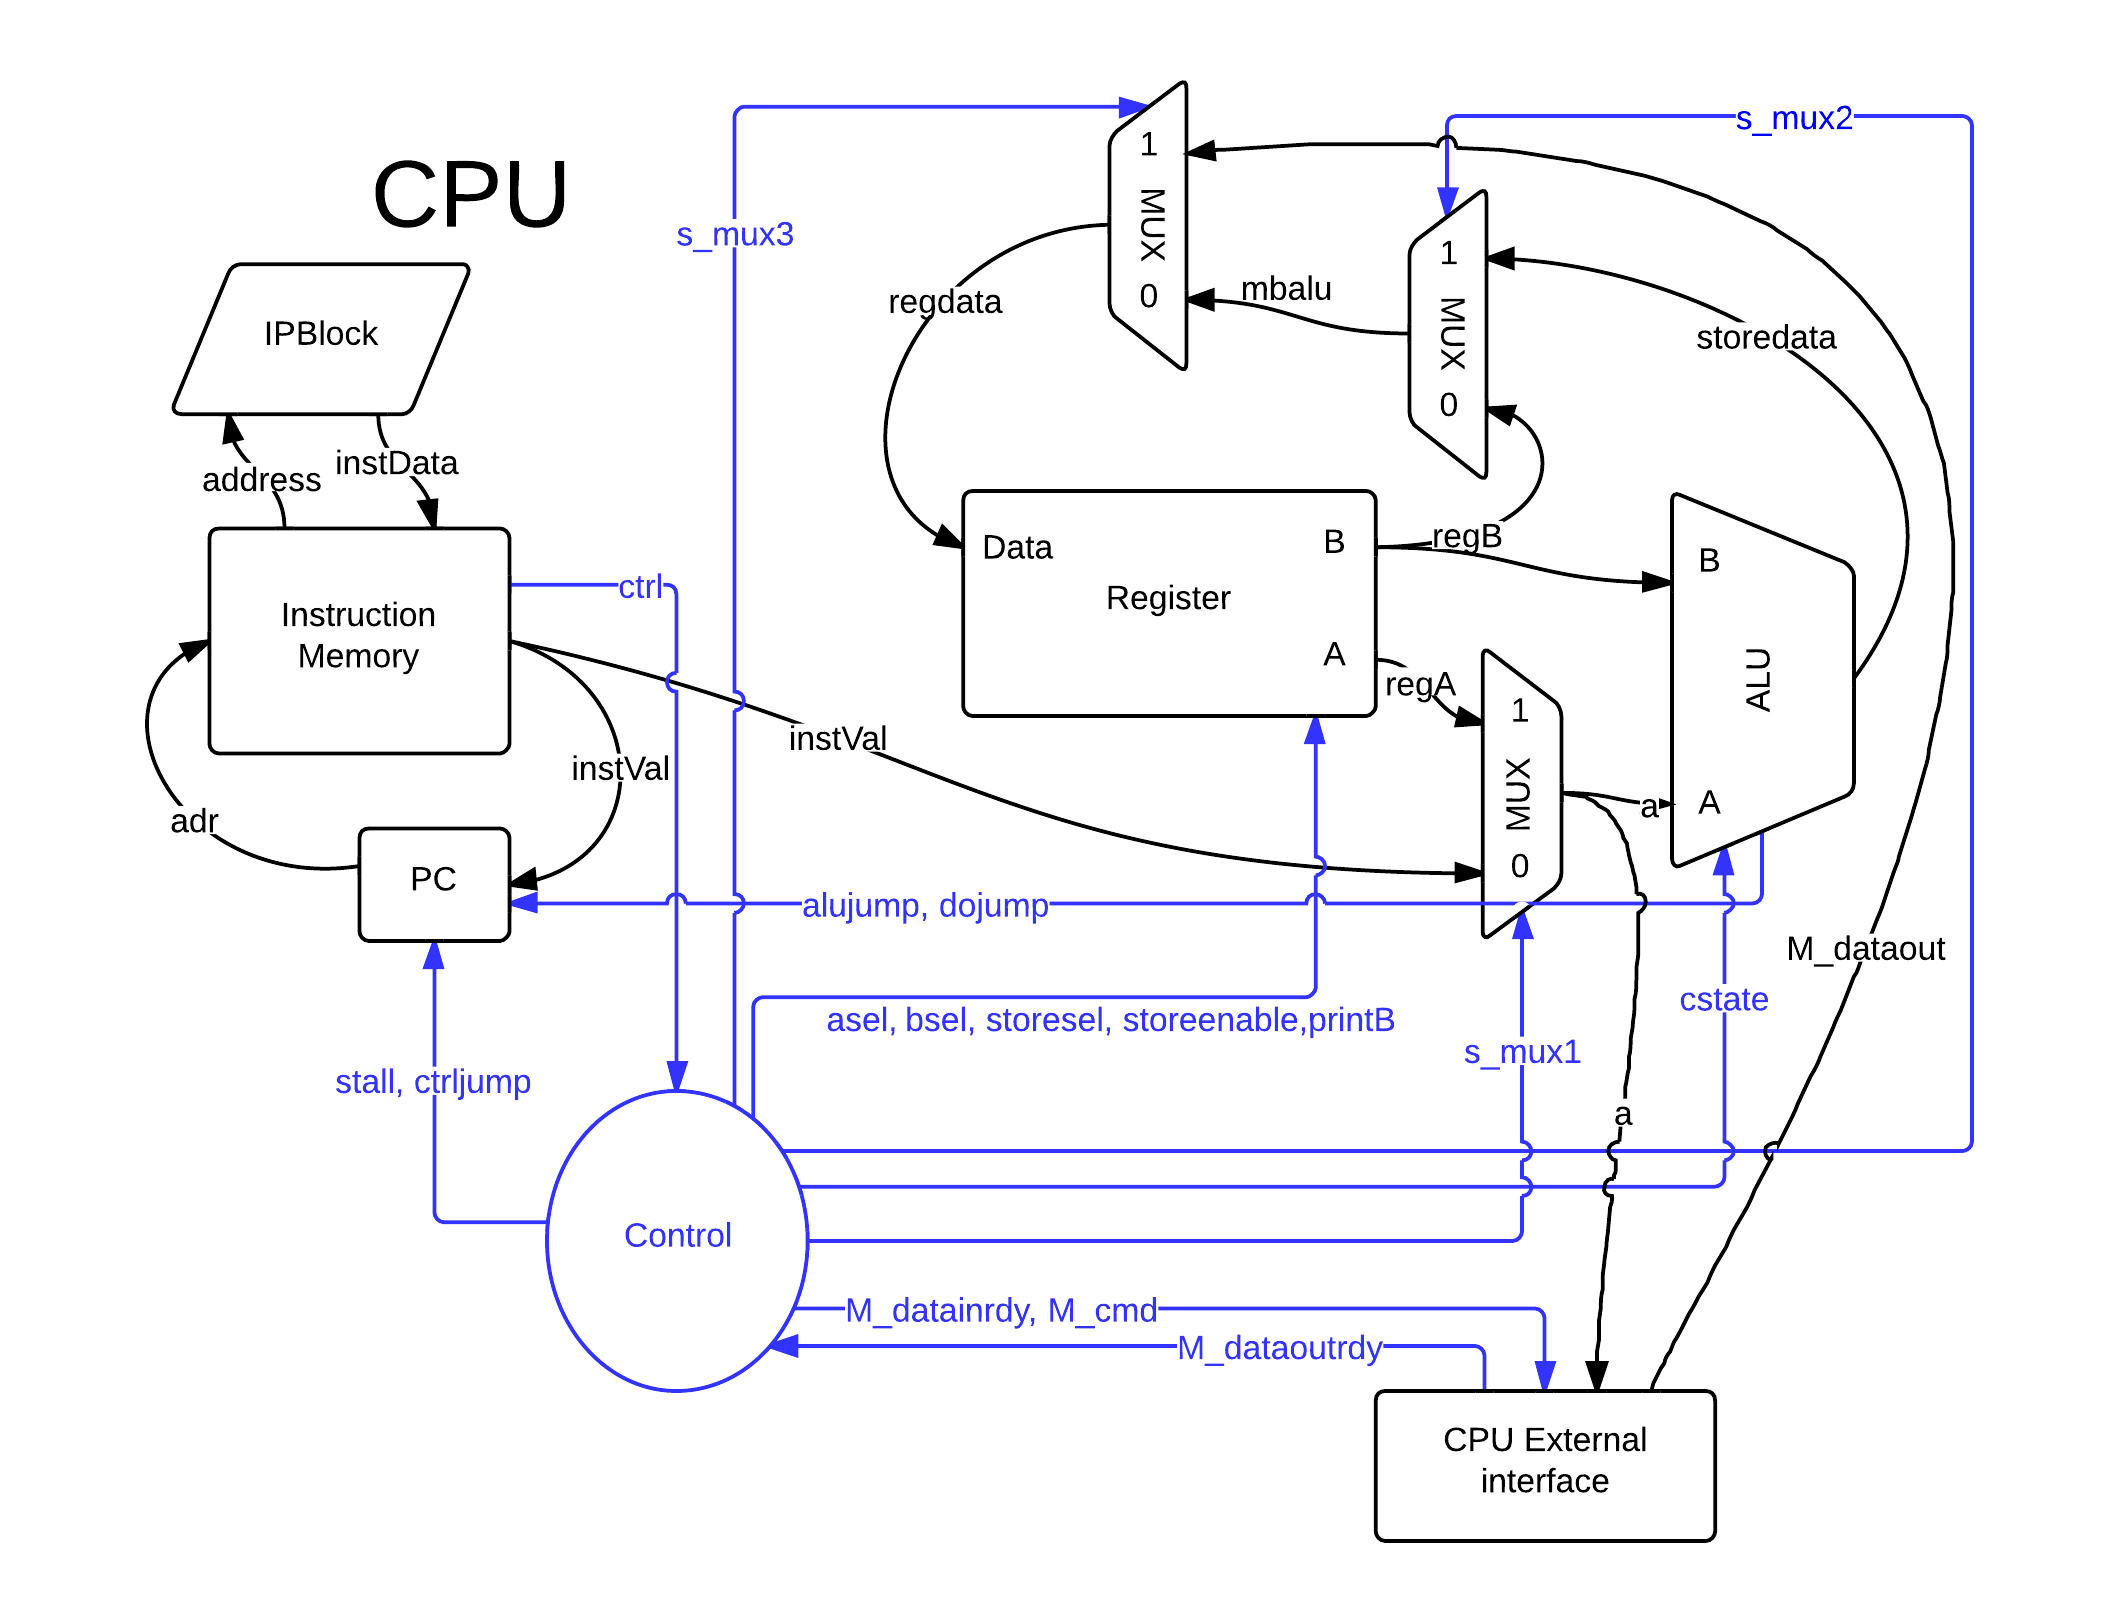
\includegraphics[width=1\textwidth]{Screenshots/CPU diagram.png}
		\caption{The Design diagram of the CPU}
		\label{DesignDiagram}
	\end{figure}

\subsection{Implementation and integration of the co-processor}

	
\section{Performance analysis}
	As can be seen in the output of which commands are run when during the course of the calculations (\ref{Commands}), it can be seen that every time a LOAD command is initiated, 8 NOP (No-Operations) follows, each taking a single clock cycle. This clearly shows that Load commands do take a lot of time and calculation and therefore, reducing them as much as possible was crucial if the processor were to reach the computation power necessary to calculate 250 data points per second. Furthermore, the list of commands also shows that communication on the bus also takes 8 clock cycles (as seen by looking at the command SCMD and the following 8 NOP commands carried out before the next calculation) - this is clearly another slow process that should be optimized as much as possible if the processor were to reach its target, speedwise.\\ %699 nops contra 301 rest
	Interestingly enough, out of a 1000 clock cycles, 699 clock cycles were spent on waiting for LOAD commands or bus communication, and only 301 clock cycles were spent on actual calculations, clearly showing just how much time it actually takes to communicate over the bus.\\
	\\
	The above, however, is not something that will be optimized upon in this report, as the time needed to do the LOAD commands are decided upon by Gezel and the fact that the co-processor must work on the bus means both must run their due courses. The rest of the operations, however, can be optimized and analysed. These 301 clock cycles consist of sequences of $1 addition \rightarrow 1 subtraction \rightarrow 1 multiplication \rightarrow 1 bitshifts$. In total, each sequence only takes a single clock cycle due to the fact that both additions, subtractions and bitshifts are very fast operations. Furthermore, this report does not require any looping through values, as described in section \nameref{Functionality}, thus making the actual critical path very short.\\
	%Skriv noget om tidsm�ngden kr�vet til at lave Critical Path
	\\
	In terms of size, this report has done very little to optimize it, but the size of the processor still remains very small as there are no loops in the co-processor, nor are the 30 previous values actually stored. As such, the size of the co-processor is equal to the sum of the bitsize of every signal used in the co-processor, and in total, that amounts to $7*32+2*16=$ bits.
	\\
	Finally, in terms of power, the interesting thing to look at is the amount of toggles - these can be seen on \ref{Toggles}.
	
		\begin{figure}[h!]
			\centering
				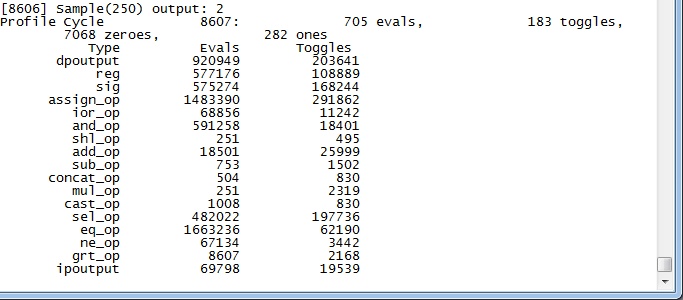
\includegraphics[width=1\textwidth]{Screenshots/Screenshot_Profiling.png}
			\caption{The Design diagram of the CPU}
			\label{Toggles}
		\end{figure}
	

\section{Discussion}
%Write all things bus-related here

	\subsection{Improvements}
		One improvement could be to implement simultaneous loading and data passing - that is, that the processor would be able to pass the data to the co-processor and then immediately start loading the next data point, as this is the process that takes the longest (8 clock cycles in Gezel). This could be done by implementing a dataStart and a dataEnd signal, used to synchronize the processor and the co-processor so the co-processor doesn't start to pass data back to the processor while the processor is loading the next data point.\\
		\\
		Alternatively, another improvement could be to implement the co-processor such that it would communicate directly with the processor, rather than using a bus. This would free up the bus to be used for the processors loading while the data is passed directly between the processor and co-processor.\\
		\\
		Furthermore, the co-processor could be improved more in terms of speed by storing the previous 30 values used for computation in the co-processor itself, rather than loading the old data. This would increase the size of the co-processor, but as this report focuses on improvements in terms of speed, this increase in size would be acceptable, considering that it remove a Load command which in itself takes 8 clock cycles (which is quite a great deal, considering that calculating an entire data point takes 35 clock cycles with the current operations).\\
		\\
		Improvements in terms of size could also be made by making a few assumptions, much like the one done with the data signal that goes between the processor and co-processor, but as this report focuses mainly on improving the speed, these have not been implemented yet. These improvements would simply be to reduce the bitwidth of various registers.\\
		

\section{Conclusion}

\newpage
\begin{thebibliography}{9}

\bibitem{A3}
  Michael Reibel Boesen, Jan Madsen, Linas Kaminskas, Karsten Juul Frederiksen, Thomas K. Malowanczyk\\
  \emph{Assignment 3: Implementation of an ECG co-processor}\\
  2013.\\

\bibitem{Gezel}
  \emph{Lecture7: Finite state machine with Datapath}\\
  Fall, 2007.\\

\bibitem{GezelBasicSyntax}
  \emph{GEZEL Basic Syntax}\\
  
\bibitem{ClockSpeeds}
  \emph{http://smallbusiness.chron.com/ghz-mean-computer-processor-66857.html}
  Used to explain clock speeds of a processor
  
\bibitem{CoreI5}
  \emph{http://www.intel.com/content/www/us/en/processors/core/core-i5-processor.html}
  Used to determine clock speeds of Core I5
  
\end{thebibliography}
	
\newpage	
	\begin{Large}
		\textbf{Appendix}
	\end{Large}
	\appendix

\section{Who wrote what}
\underline{Jacob Gjerstrup, s113440 wrote:}\\
\textbf{Report:}\\
\textbf{Code:}
\\
\underline{Jakob Welner, s124305 wrote:} \\
\textbf{Report:}\\
\textbf{Code:}

\section{Data files}
	\lstinputlisting[language=Python]{Code/showCmds.txt}
	\label{Commands}

\section{Sourcecode}

\subsection{Source code}
	\subsection{Assembly code}
		Python code:
		\lstinputlisting[language=Python]{Code/assembler.py}
		
		Assembler code for the program:
		\lstinputlisting{Code/assembler_program.txt}	
	
	\subsubsection{Co-processor}
		\lstinputlisting[language=C]{Code/coprocessor.fdl}
		
	\subsection{Platform code with co-processor integrated}
		\lstinputlisting[language=C]{Code/Platform.fdl}
	
	\subsection{Hexcodes for the program}
		\lstinputlisting{Code/program.txt}
\end{document}